\documentclass[a4paper,utf8]{article}
\usepackage[heading,fancyhdr]{ctex}
\usepackage{amsmath,amssymb,geometry,lastpage,ulem}
\usepackage{array,tabularx,graphicx,floatrow}
\geometry{
    top=25.4mm, 
    left=30mm, 
    right=30mm, 
    bottom=35mm,
    headsep=5.9mm,
}
\ctexset{
    section = {format+=\raggedright}
}
\newcommand{\expinfo}[5]{
    {\zihao{-3}\bfseries\songti
    实验名称:\uline{\hfill\mbox{#1}\hfill} \\[2.9mm]
    学\quad 号:\uline{\makebox[25mm]{#2}}\hfill
    姓\quad 名:\uline{\makebox[25mm]{#3}}\hfill
    班\quad 级:\uline{\makebox[25mm]{#4}} \\[2.9mm]
    合作者:\uline{\makebox[25mm]{无}}\enspace~
    桌\quad号:\uline{\makebox[25mm]{}}\hfill\mbox{}\\[2.9mm]
    指导教师:\uline{\makebox[30mm]{#5}}\hfill\mbox{} \\[2.9mm]
    实验日期:\uline{\makebox[30mm]{}}\hfill\mbox{} \\[58.7mm]
    }
}%\expinfo{实验名称}{学号}{姓名}{班级}{指导教师}
\pagestyle{fancy}
\fancyhf{} \fancyhead[C]{材料科学基础实验} \fancyfoot[C]{\thepage~/~\pageref{LastPage}}
\begin{document}
\begin{center}
    {\mbox{}\\[7em]\zihao{2}\bfseries\songti%
    材料科学基础实验报告}\\[34mm]
    \expinfo{实验三 碳钢退火、正火后的组织观察与硬度分析}{22301070}{杨雨燃}{22材物}{杨玉华}
    {\zihao{4}\bfseries\songti
    实验考核\\[3mm]
    \extrarowheight=3mm
    \begin{tabularx}{150mm}{|X|X|X|X|X|}\hline
        \hfil 项目 \hfil  & \hfil 实验预习 \hfil & \hfil 实验过程 \hfil & \hfil 分析与讨论 \hfil & \hfil 总评 \hfil \\[3mm] \hline
        \hfil 评价 \hfil &  &  &  &  \\[3mm] \hline
    \end{tabularx}
    }
\end{center}
\newpage
\section*{【实验目的】}
    \begin{enumerate}
        \item 了解碳钢的退火、正火过程。
        \item 观察和研究碳钢经不同退火处理、正火处理后显微组织的特点,分析热处理工艺对其组织与硬度的影响,并了解退火、正火的应用领域。
    \end{enumerate}   
\section*{【实验原理】}%简单描述,含必要的公式和附图;
\textbf{(一) 退火}

退火处理是将工件加热到适当温度并保温, 然后进行缓慢冷却的热处理方法。其目的是使工件内部组织达到或接近平衡状态,获得良好的工艺性能和使用性能,或者为进一步淬火过程作组织准备。

1.完全退火(加热至 $A_3+30 \sim 50$°C)
主要用于消除毛坯件中的魏氏组织、带状组织等组织缺陷,调整硬度、改善切削加工性能。

2.不完全退火(加热至 $A_1 \sim A_3$°C)
主要目的是降低硬度、改善切削加工性、消除内应力;
特点为加热温度低,消耗热能少,降低工艺成本。

3.球化退火(加热至$A_1+20$°C)
降低硬度、改善切削加工性、改善组织、提高塑性等。

4.去应力退火(加热到相变点 $A_1$ 以下的某一温度)
消除由于冷热加工所产生的残余应力。

5.扩散退火(加热至 $A_3$ 或 $A_{cm}$+150$\sim $300°C)
又称均匀化退火,用于合金钢锭和铸件。以消除枝晶偏析,使成分均匀化。

\textbf{(二)正火}

正火处理与一般退火的不同之处在于试样在空气中以稍大的冷却速度中进行冷却。由于正火冷却速度较快,过冷度较大因而发生伪共析组织转变,使组织中珠光体量增多,且珠光体的层片厚度减小,故得到精细结构。
这时所获得的组织为索氏体 S 或屈氏体 T 属珠光体类型,是铁素体和渗碳体的混合物。用于消除过共析钢中的网状二次渗碳体,为进一步的球化退火作好组织准备。

\textbf{(三)退火与正火加热温度选择}

\begin{center}
    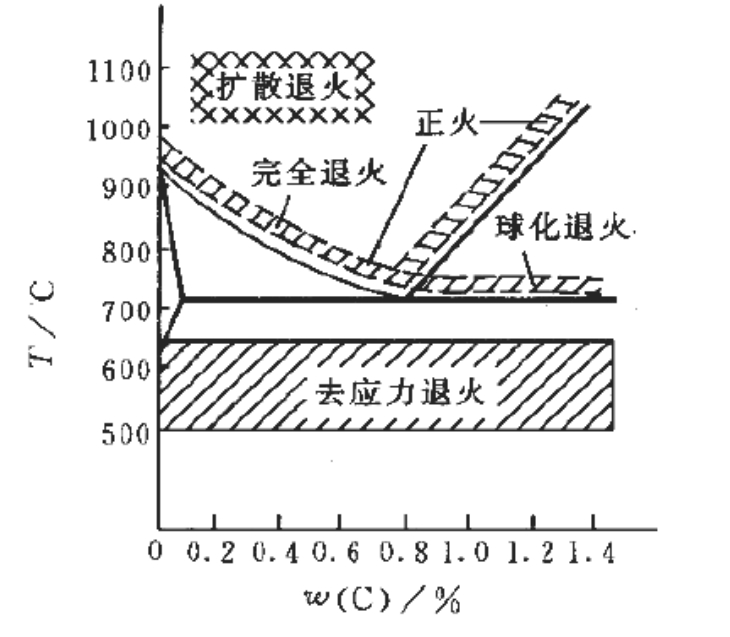
\includegraphics[width=200pt]{1.png}
\end{center}

上图是退火和正火的加热温度范围图。

\textbf{(四)退火与正火保温时间的确定 }

 τ = KD

式中,K为加热系数,一般K=1.5$\sim$2.0min/mm;D为工件有效尺寸。装炉量不大时可以使用此式。


\textbf{(五)显微组织的观察}

若白色网状组织比较粗大,且粗细不均匀,并且还能清楚看到网状组织中存在黑色细而均匀的线条(即晶界),则可以判断该组织为铁素体;若白色网状组织很细很均匀,则可判断为网状二次渗碳体。

亚共析碳钢一般采用完全退火,经退火后可得接近于平衡状态的组织,即铁
素体加珠光体。T12钢经球化退火后组织为球状珠光体。
二次渗碳体和珠光体中的渗碳体都呈球状(或粒状),左图。45钢正火组织
为铁素体+索氏体如右图。
\begin{center}
    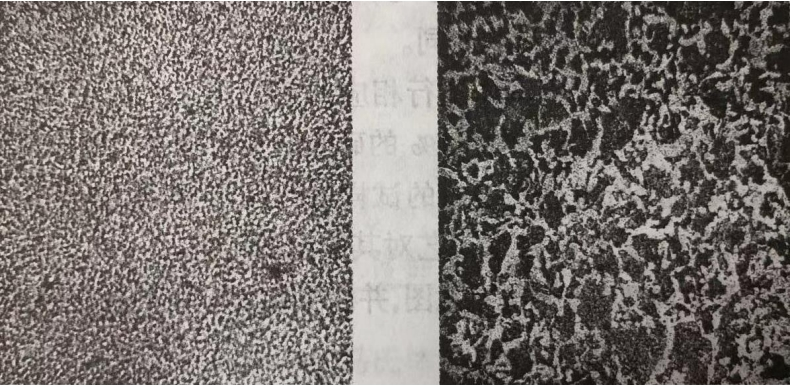
\includegraphics[width=350pt]{2.png}
\end{center}
\section*{【实验仪器】}%规格及参数
箱式电阻加热炉,洛氏硬度计,砂纸,抛光机,金相显微镜。热处理试样:
45钢及T12钢。
\section*{【实验过程】}%简述主要过程和实验内容
1、4人一组,45钢(2个)、T8(1个)及T12钢(1个),(对应下表中相应的热处理工艺方法)

\begin{center}
    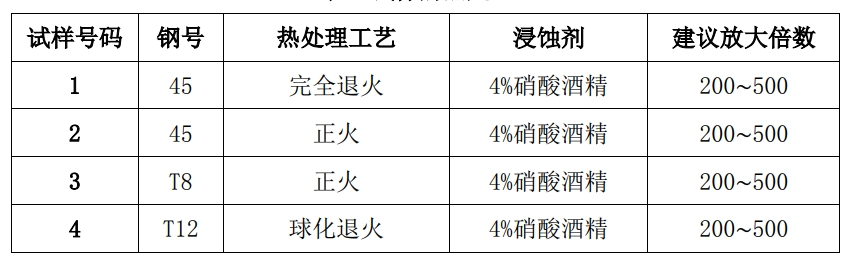
\includegraphics[width=350pt]{3.png}
\end{center}

2、制定热处理工艺参数,可参考以下工艺参数。

① 45钢完全退火工艺:加热温度为860 ± 10℃,根据试样有效尺寸计算保温
时间,保温后炉冷到500℃左右出炉空冷。

② 45钢正火工艺:加热温度为860 ± 10℃,根据试样有效尺寸计算保温时
间,保温后出炉空冷。

③ T8钢正火工艺:加热温度为820 ± 10℃,根据试样有效尺寸计算保温时间,
保温后出炉空冷。

④ T12钢球化退火工艺:加热温度为760 ± 10℃,根据试样有效尺寸计算保
温时间(约40分钟),保温后随炉冷却到680℃保温40分钟,随后炉冷到500℃出
炉空冷。

3、利用硬度计对所有热处理后的试样进行硬度测试,每个试样至少三个试验点,再取一个平均值,分析热处理工艺对其硬度的影响。按照下表选用硬度计。(硬度测试须在金相磨制观
察前完成)

\begin{center}
    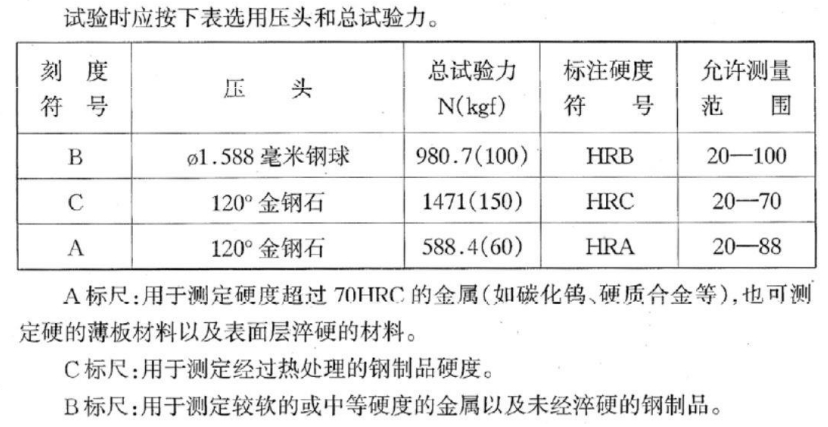
\includegraphics[width=350pt]{4.png}
\end{center}


4、根据拟定的热处理工艺对试样进行相应的热处理工艺处理,然后利用金相砂
纸对热处理后的试样进行磨制、抛光,并用4\%的硝酸酒精进行腐蚀制得金相试样。
利用金相显微镜对其进行显微组织观察,分析热处理工艺对其组织的影响。

5、实验结束后,汇总各小组实验数据,根据实验数据分析冷却方法对碳钢性能(硬度)的影响,并阐明硬度变化的原因。

\newpage

\section*{【实验数据及处理】}

\begin{table}[!ht]\centering
    \caption{不同热处理试样的硬度}
    \extrarowheight=11pt
    \begin{tabularx}{\textwidth}{|c|X|X|X|X|}\hline
        材料及热处理状态 & \multicolumn{3}{c|}{测得硬度数据} & \hfil 平均值 \hfil \\[10pt] \hline
        45 钢经完全退火 & 82.0HRB & 83.6HRB & 79.6HRB & 81.7HRB \\[10pt] \hline
        45 钢经正火 & 96.5HRB & 91.0HRB & 92.5HRB & 93.3HRB \\[10pt] \hline
        T8 钢经正火 & 27.3HRC & 28.3HRC &26.5HRC  & 27.4HRC \\[10pt] \hline
        T12 钢经球化退火 & 93.7HRB & 93.0HRB &93.1HRB  & 93.3HRB \\[10pt] \hline
    \end{tabularx}
\end{table}

测试硬度的硬度计表盘最小分度均为0.1HRB(HRC)

因而,我们可以依照公式得到其硬度的不确定度。如下表。
公式如下:(X为硬度,$\bar{X} $为硬度的平均值)
\begin{center}\zihao{4}
    $ S = \frac{\Sigma |X - \bar{X}| }{3} $
\end{center}

\begin{table}[!ht]\centering
    \caption{不同热处理试样的硬度以及不确定度}
    \extrarowheight=11pt
    \begin{tabularx}{\textwidth}{|c|X|X|X|X|}\hline
        材料及热处理状态  & \hfil 平均值 & \hfil 不确定度  \\[10pt] \hline
        45 钢经完全退火 & \hfil 81.7HRB &\hfil1.4HRB \\[10pt] \hline
        45 钢经正火  & \hfil 93.3HRB & \hfil2.1HRB \\[10pt] \hline
        T8 钢经正火  & \hfil 27.4HRC &\hfil0.6HRC \\[10pt] \hline
        T12 钢经球化退火 & \hfil 93.3HRB &\hfil0.3HRB \\[10pt] \hline
    \end{tabularx}
\end{table}

分析:

1.对于45钢,完全退火的45钢相比正火的45钢,硬度更小,说明,在更慢的降温速度下,过冷度更低,正火可以获得更细密的结构,从下面的图片以及正火原理也可以看出。
因而其力学性能相较完全退火的45钢更好。这也与理论相符。

2.按照碳含量来看,从45钢,到T8钢,T12钢,其原本的硬度就有一定递增关系,其中T8钢相比45钢(同为正火工艺),硬度更高,HRC标尺所表示的硬度比HRB的标尺的硬度更高。

3.正火和球化退火和完全退火,三种不同的工艺,原理上有很大的不同,从下面对于结构的分析中可以看出。我们可以看出,球化退火的钢相比正火的T8钢更软,相比正火45钢更硬,
同时T12钢原本是三者最硬的,这间接说明,球化退火工艺有更好的韧性,更低的硬度,这与理论相符。

\section*{【实验图像记录】}
1.下面图1图2是45钢完全退火的图片:

\begin{figure}[!ht]
    \begin{floatrow}
        \ffigbox[60mm]{\caption{45钢完全退火1}}{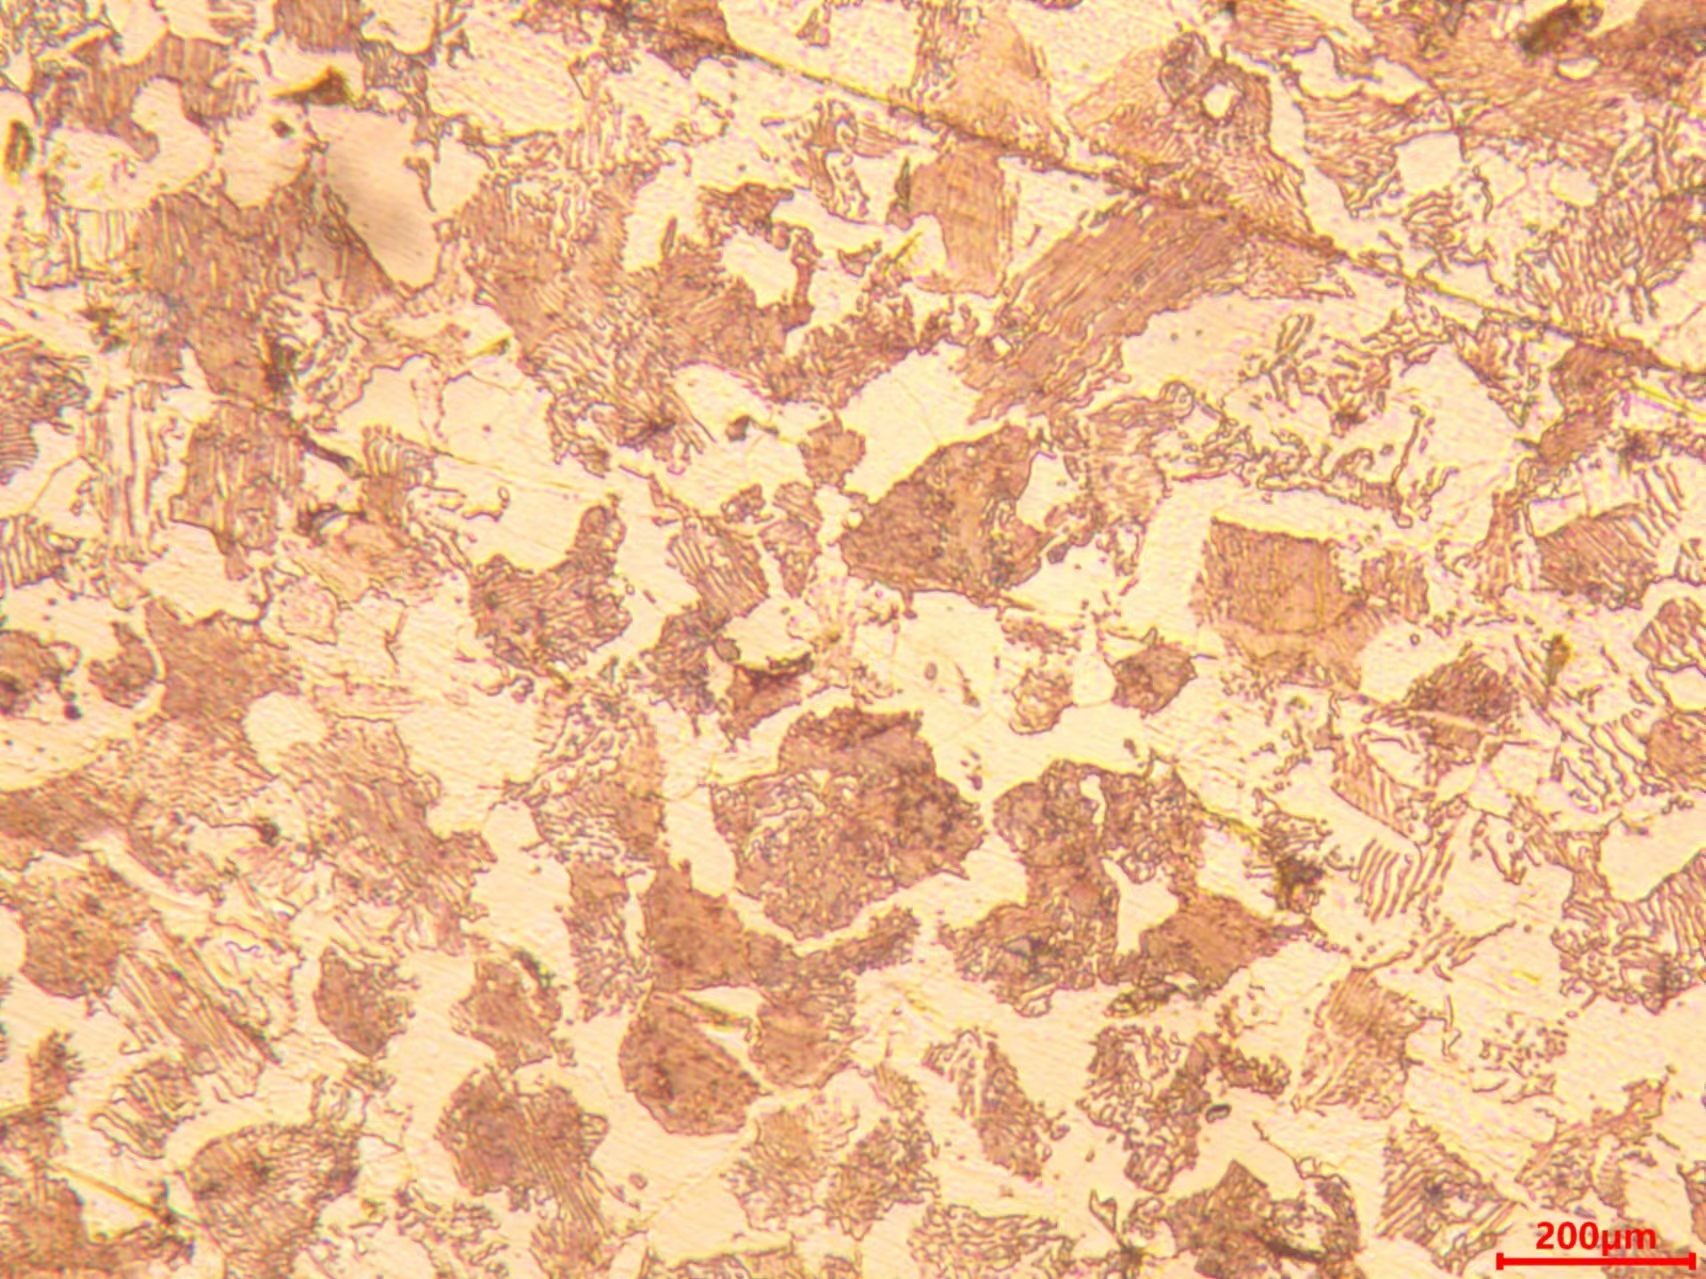
\includegraphics[width=60mm]{111.jpg}}
        \ffigbox[60mm]{\caption{45钢完全退火2}}{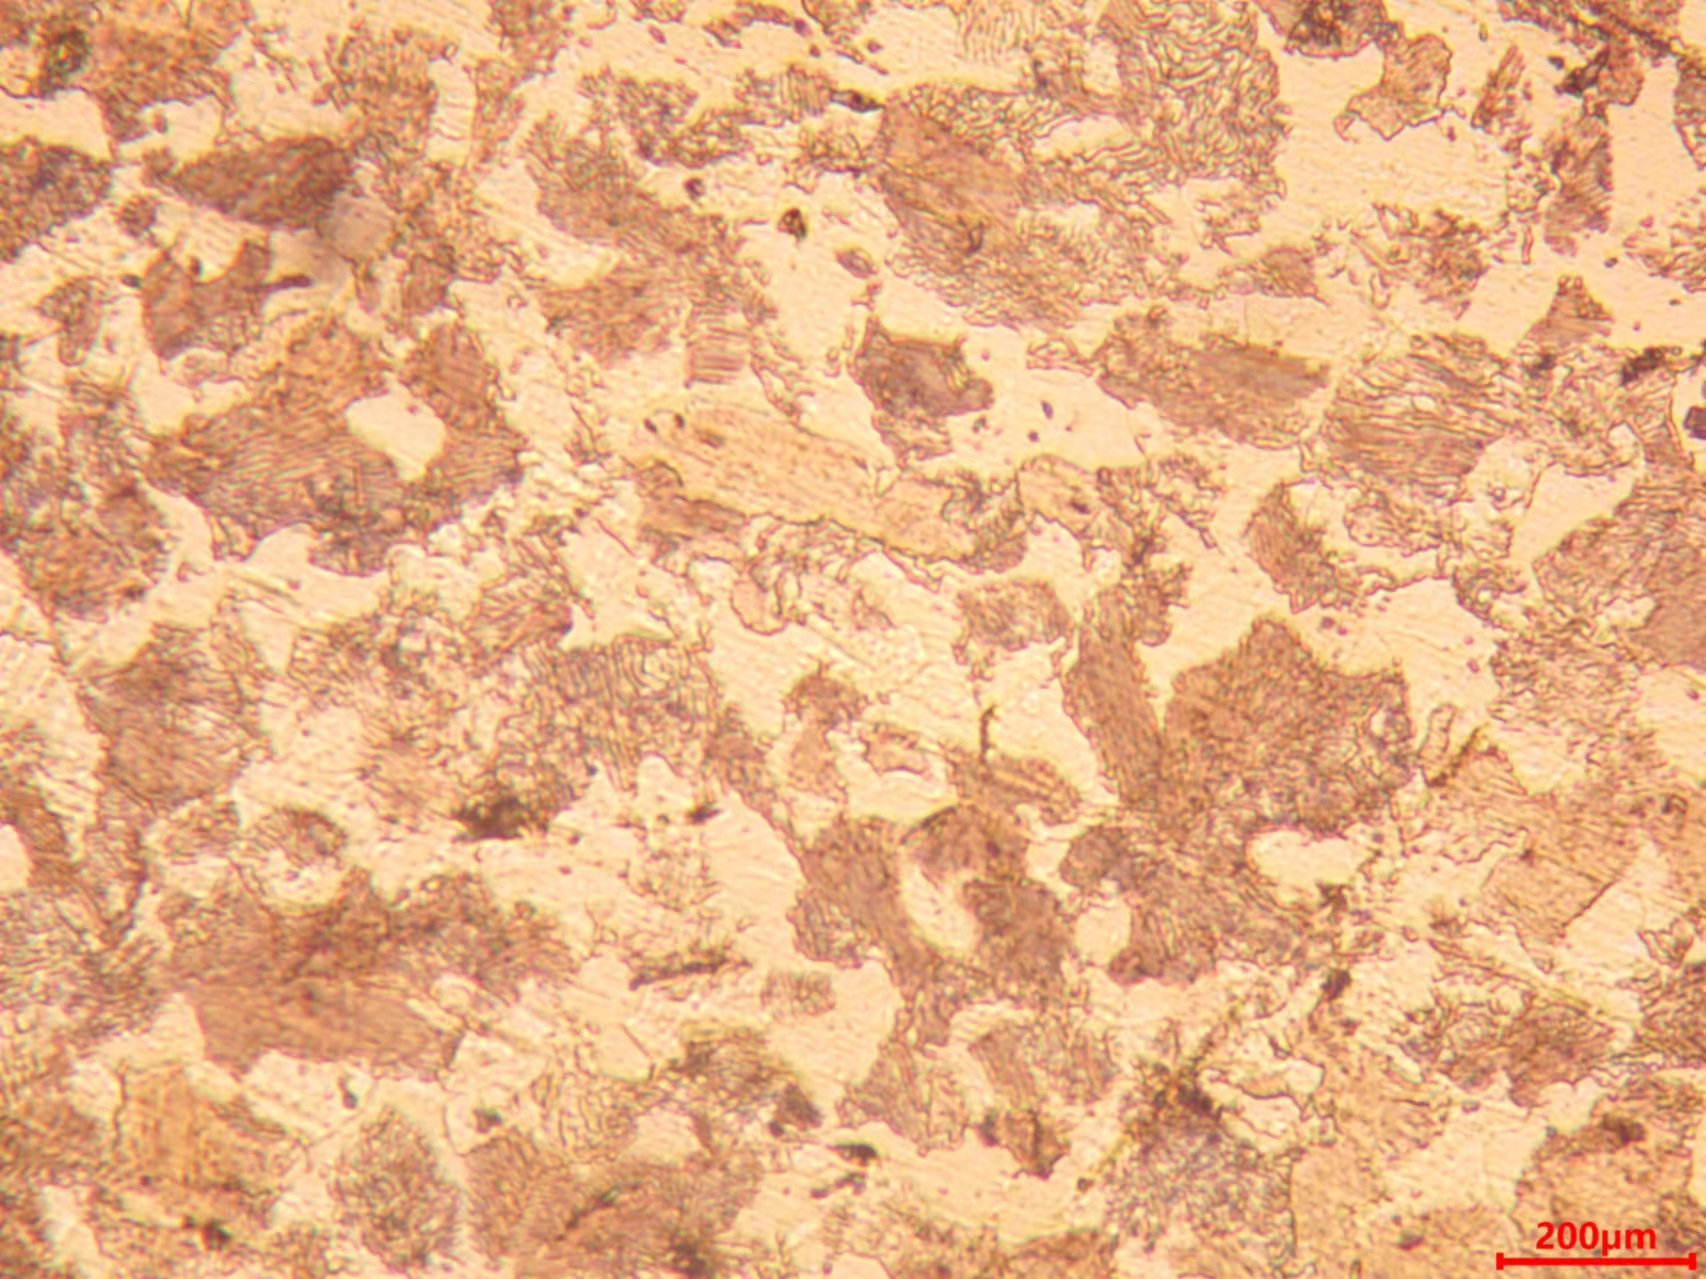
\includegraphics[width=60mm]{112.jpg}}
    \end{floatrow}

\end{figure}

分析:45钢完全退火的微观结构主要为铁素体加上珠光体,从图中可以看出,相对明亮的区域是铁素体,暗的区域是珠光体,整体较为平衡,组成相对稳定,
珠光体呈现片状,例如在图一的右下方有细条状间隔的铁素体和渗碳体。其整体较小,比一块片状珠光体小。

\newpage

2.下面图3是45钢正火后的图片:

\begin{figure}[!ht]
    \begin{floatrow}
        \ffigbox[60mm]{\caption{45钢正火1}}{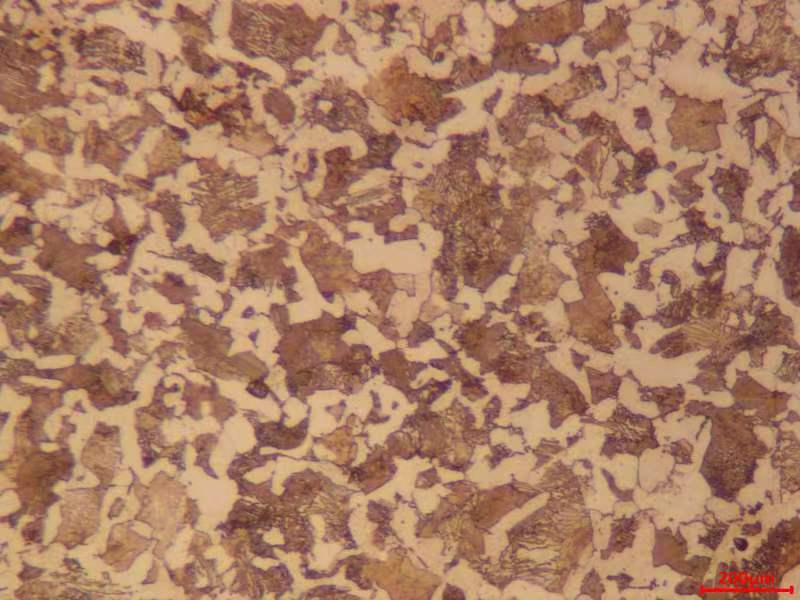
\includegraphics[width=60mm]{121.jpg}}
    \end{floatrow}

\end{figure}

分析:正火时,相对于退火更快速地冷却,过冷度较大因而发生伪共析组织转变,使组织中珠光体量增多,且珠光
体的层片厚度减小,这时所获得的组织为索氏体 S 或屈氏体 T 属珠光体类。
型,是铁素体和渗碳体的混合物。

由图3,亮色地条状结构为铁素体,暗的区域是珠光体类,大致为索氏体,相比退火的图片,珠光体(索氏体)更为细小,而布呈现明显的大片状。

3.下面是T8钢正火后的图片:

\begin{figure}[!ht]
    \begin{floatrow}
        \ffigbox[60mm]{\caption{45钢正火1}}{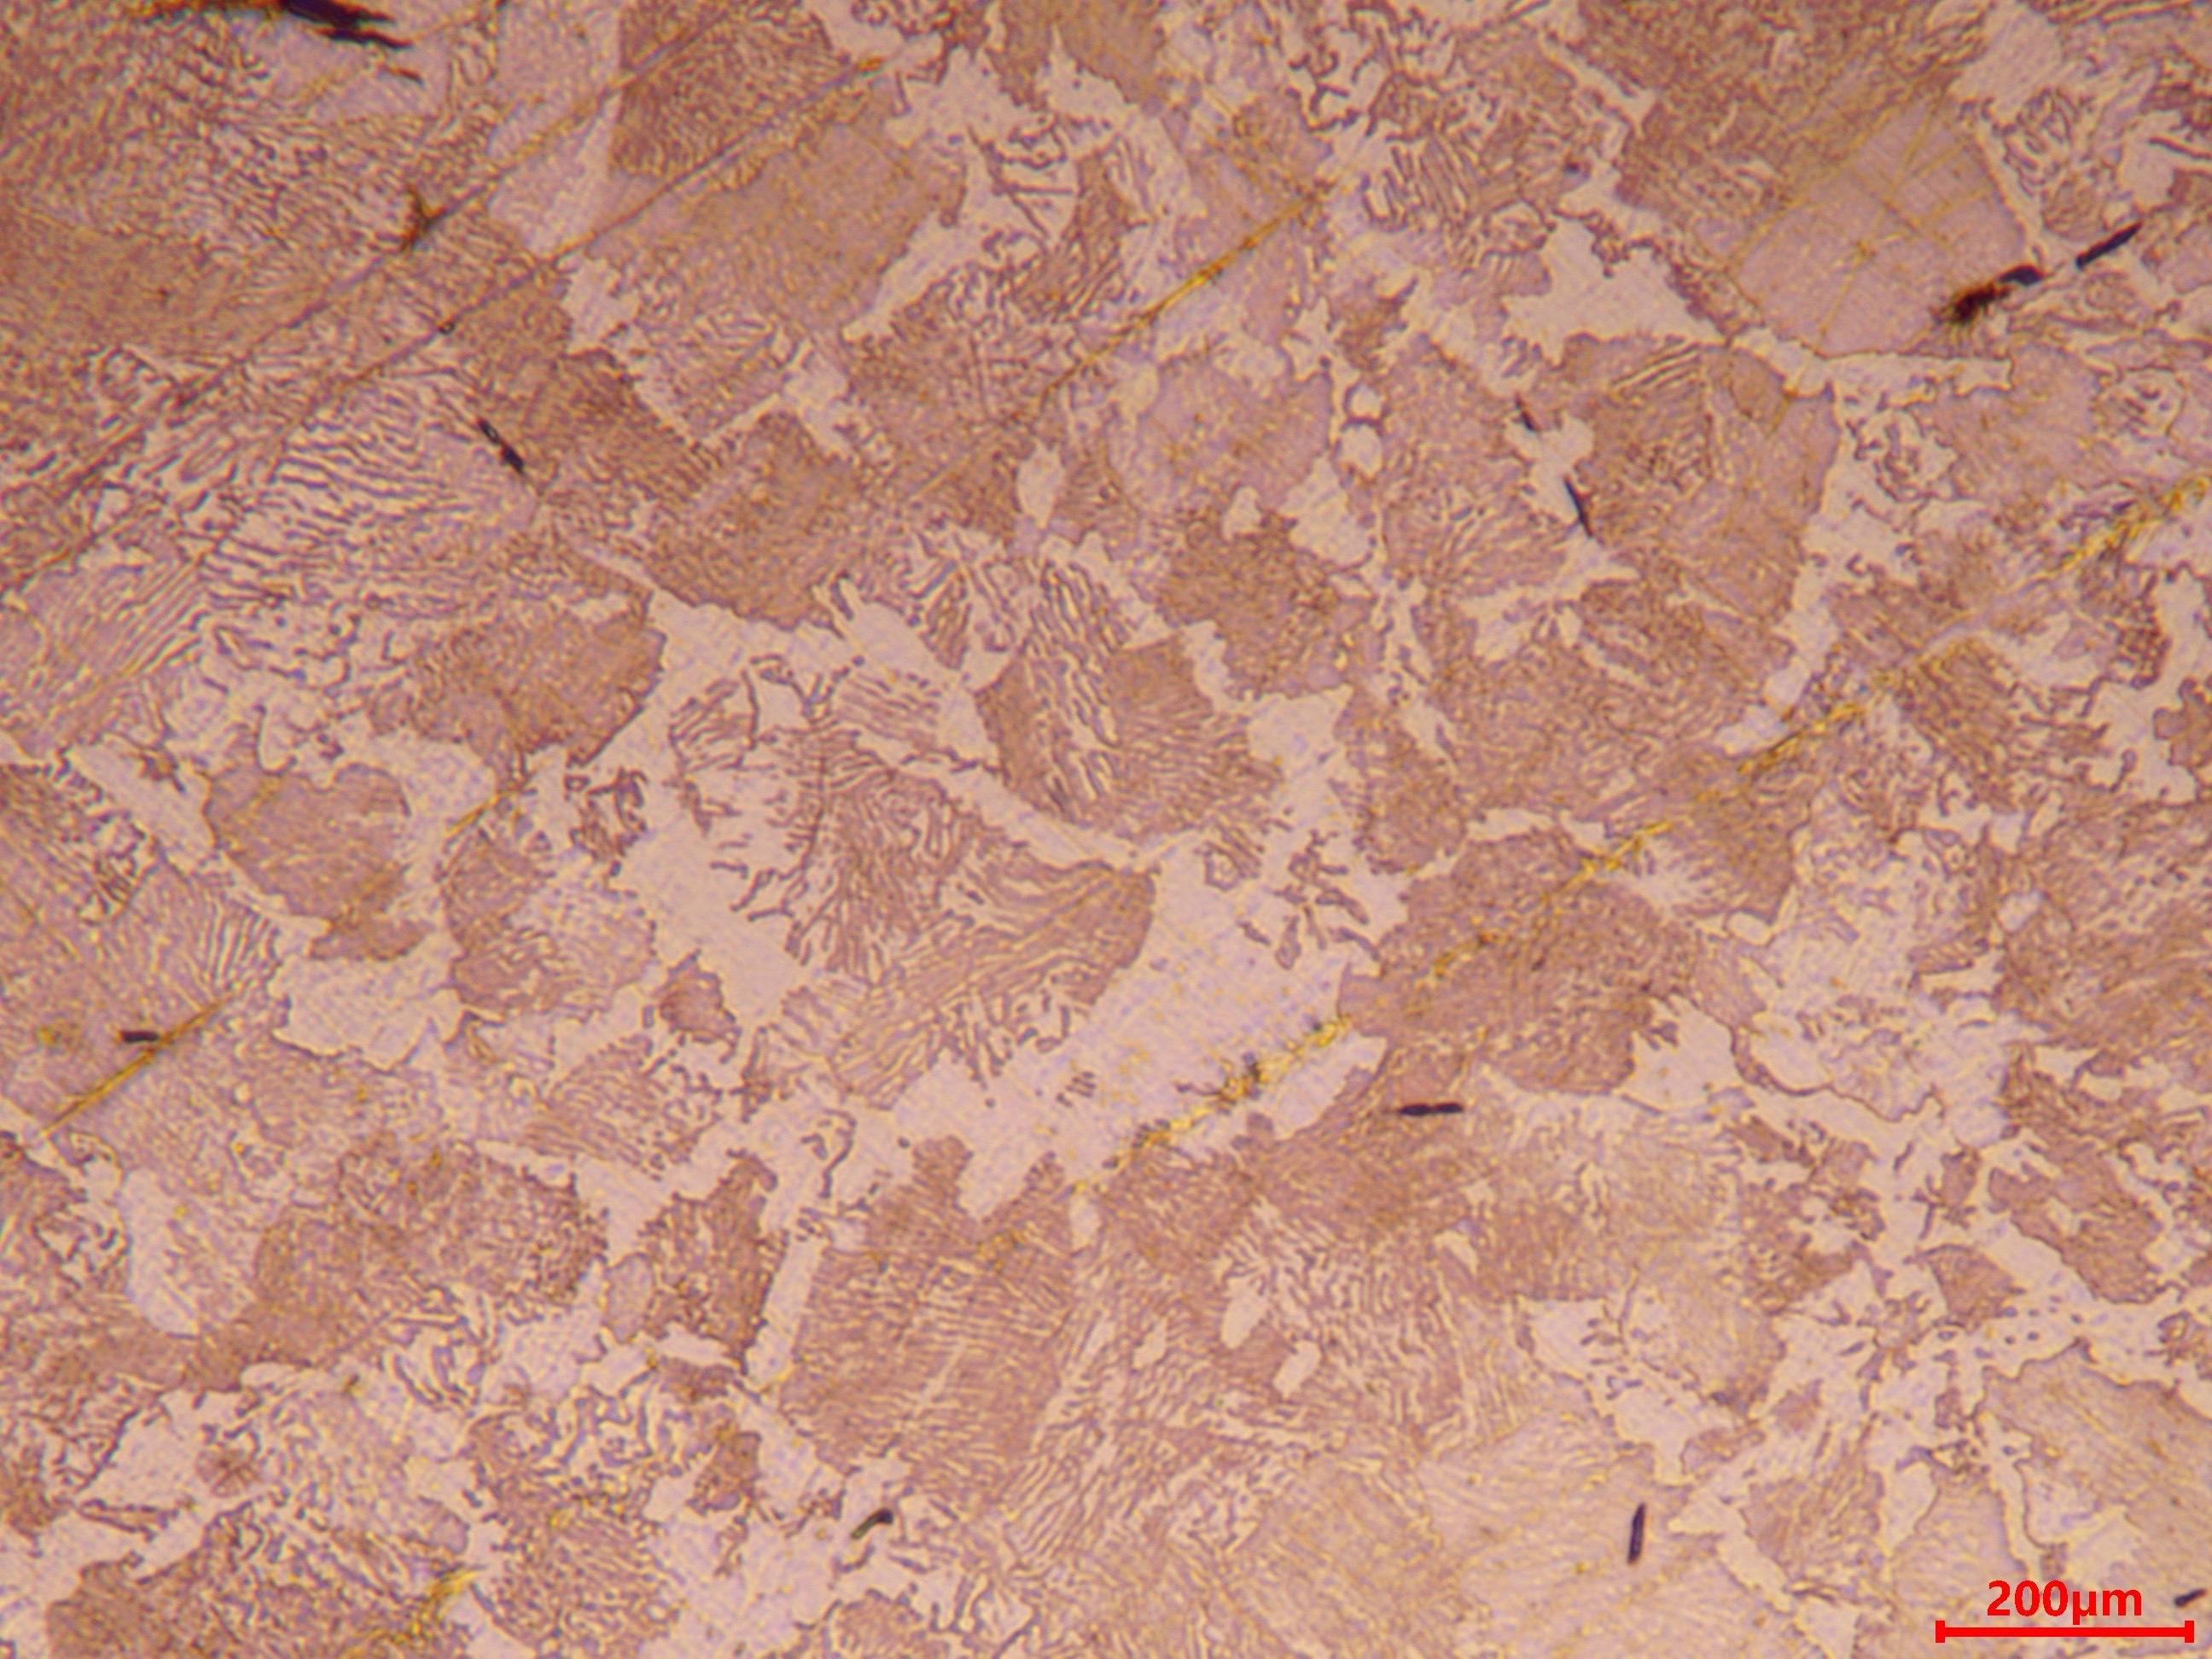
\includegraphics[width=60mm]{131.jpg}}
    \end{floatrow}

\end{figure}

分析:图4,亮色(白色)部分为铁素体,黑色部分为块状的索氏体。相比45钢正火的图片,索氏体的占比明显增多,且多
呈现更大的块状,但在与铁素体交接的部分有更多的相互交织渗透,呈现细条状。

4.下面是T12钢球化退火后的图片:

\begin{figure}[!ht]
    \begin{floatrow}
        \ffigbox[60mm]{\caption{45钢正火1}}{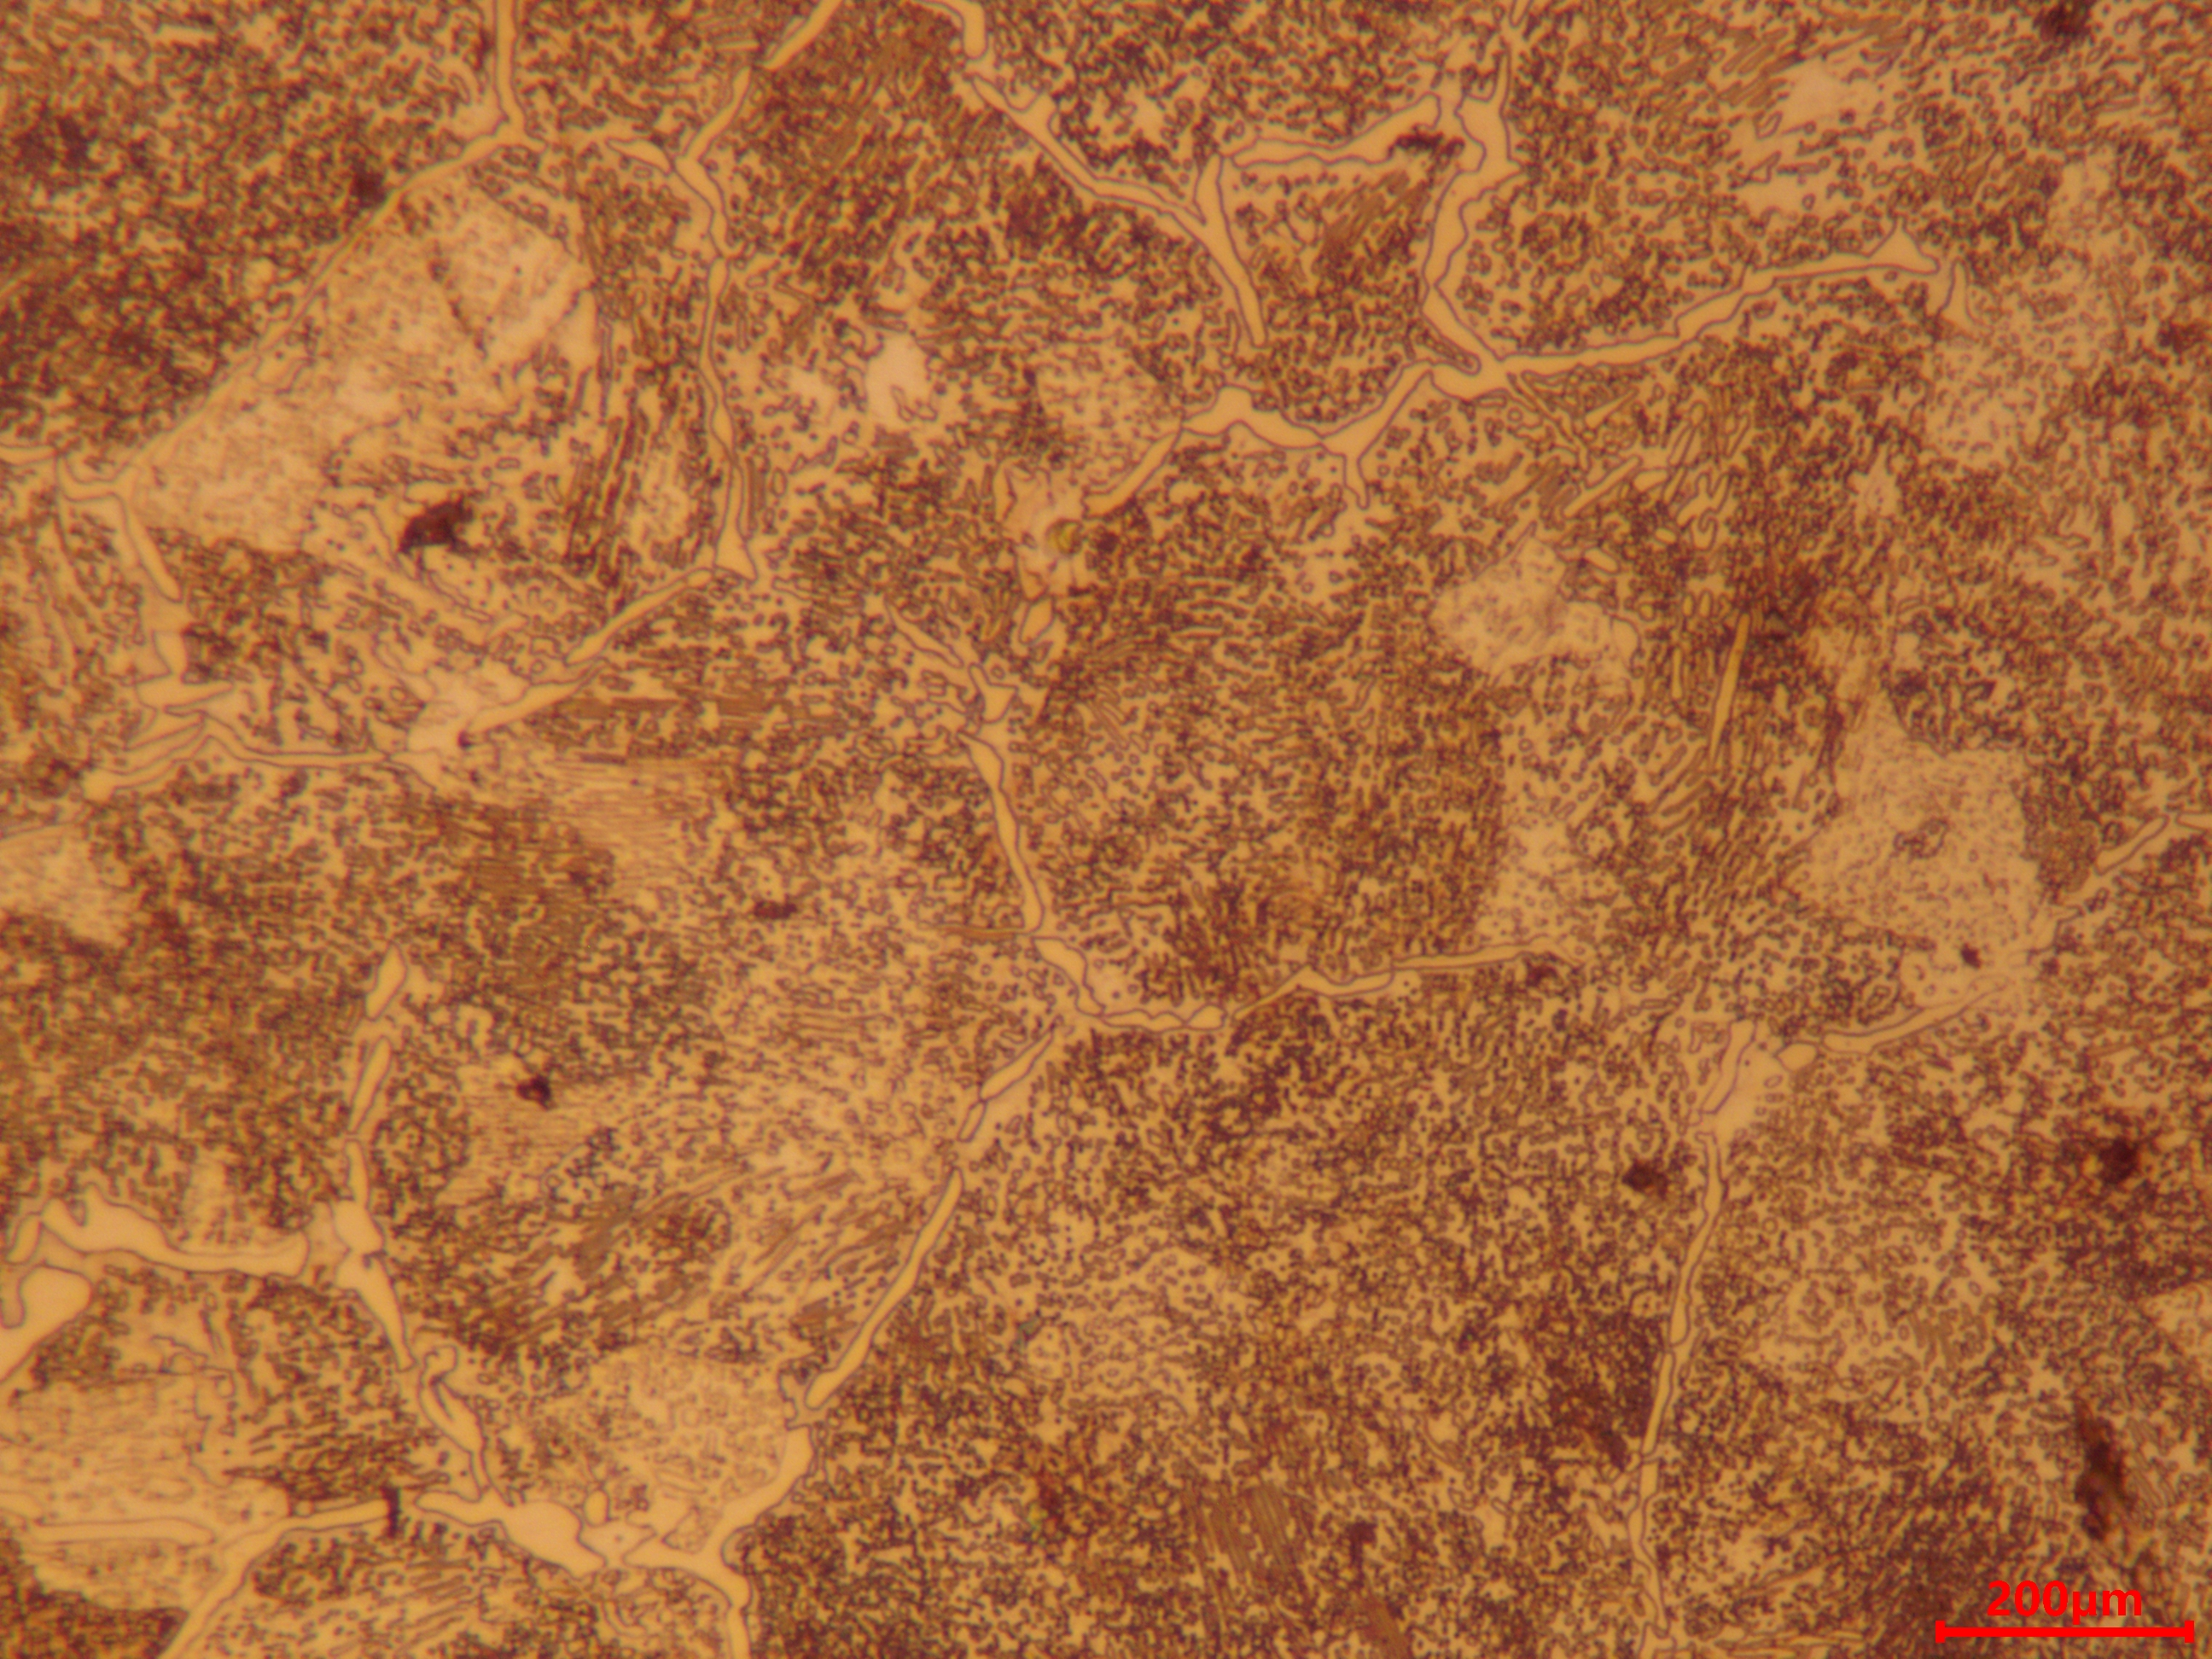
\includegraphics[width=60mm]{141.jpg}}
    \end{floatrow}

\end{figure}

分析:观察图5我们可以看出,其组织主要为球状的珠光体(暗色区域)。珠光体,渗碳体基本都呈现处球状或者粒状,
然后堆积成相对大的整体,在基体上有分散的白色颗粒状物质分布。

\section*{【思考题】}

1.45钢工件常用的热处理是:先正火、再调质、最后进行表面高频淬火和低温回火。正火后的组织为铁素体和索氏体,硬度为170HRB $\sim $200 HRB ;调质处理后的组织为回火索氏体,硬度为28$\sim $35HRC;表面高频淬火和低温回火后组织为表面为极细的回火马氏体,中心部为回火索氏体。
不同热处理方式的45钢,性能不同,用途也不同。若采用上述方法,先退火,调质,淬火,高温回火得到回火索氏体。其可以用于经常受到强负荷或者应力的部件,例如螺栓,螺丝,连杆,齿轮。

2.将亚共析钢件加热到$A_3$+(30 $\sim$ 50)℃($A_3$线是钢$\alpha$ 固溶体转变为$\gamma$ 固溶体之临界温度),保温一段时间,由于退火温度大致为860摄氏度,后面直接水冷淬火操作,钢淬火的主要目的是为了获得马氏体,提高它的硬度和强度,低温时铁素体较多,淬火后硬度不高,温度过高时会出现更多片状的,大的马氏体,相对硬度也会下降。因而大致上硬度随温度先升高,后降低,峰值在860摄氏度左右出现。

3.经过球化退火的T12钢一般呈现出珠光体组织,也就是球状晶粒。球化退火可以提高钢材的塑性和韧性,同时降低硬度。球化退火后,具有较好的塑性、韧性和可加工性,适用于需要较高塑性和韧性的工程应用,但相对强度和硬度会较低。

\end{document}